\chapter{SW and HW Implementation}
\label{cha:software and hardware implementation}
The overall system will work as shown in \textbf{Figure \ref{fig:software pipeline}}:\newline 
1. The microphones capture the user's voice and save it in the buffer\newline
2. Meanwhile the buffer is being filled in the respective devices, the MFE block is being triggered and its spectrogram output is given in input to KWS segment. It will process the input in Syntiant Pipeline, meanwhile SV performing device will wait for a response.\newline
3. The KWS routine finishes and it communicates the classification output to the SV device via SPI\newline
4. The SV, according to the output, if it is a class, computes the Syntiant pipeline.\newline
5. After extraction of d-vector, the system compares the result obtained with the reference vectors of the corresponding word, limiting unnecessary comparisons.\newline\newline
The possible outputs of the system are:\newline
• No word is recognized, so the SV is not triggered and will not process the spectrogram.\newline
• The sample corresponds to a word, but the user is not enrolled for that specific class.\newline
• The sample corresponds to a word and the user is enrolled for that specific class.\newline
According to these different outputs, the programmer will be free to perform a connected action.\newline
This thesis, at first, was developed considering the system implementation on two Syntiant NDP101 devices with the objective of creating a multi-model system. Ultimately, because an NDA was not possible to deploy, the overall idea will be presented as if access to the SDK was granted.
A multi-model system consists of having a uniform signal processing with an appropriate reshape and MFE block processing by an NDP101 and only then the result will be parsed to the other device to perform a different model action.
During the dissertation of the methodology used in the software pipeline, two different approaches would have been followed:\newline\newline
• Simulation on a computer (Software Approach) - Created to verify system pipeline correctness before deployment. It does not use any hardware component, except the microphone integrated into the computer. Shows the behavior using pure C code and saving the models in header.\newline
• Inference on MCU (Software + Hardware Approach) - Actually application deployment, which requires handle of hardware components. In this case, the models are uploaded in binary files, but each one is on a different MCU, not like the simulation, which was all accessible by the same compiler. The hardware and communication (SPI) had to be managed, but the other phases are equal to the ones edited in C in the simulation.\newline
\begin{center}
    \centering
    \begin{figure}[!h]
        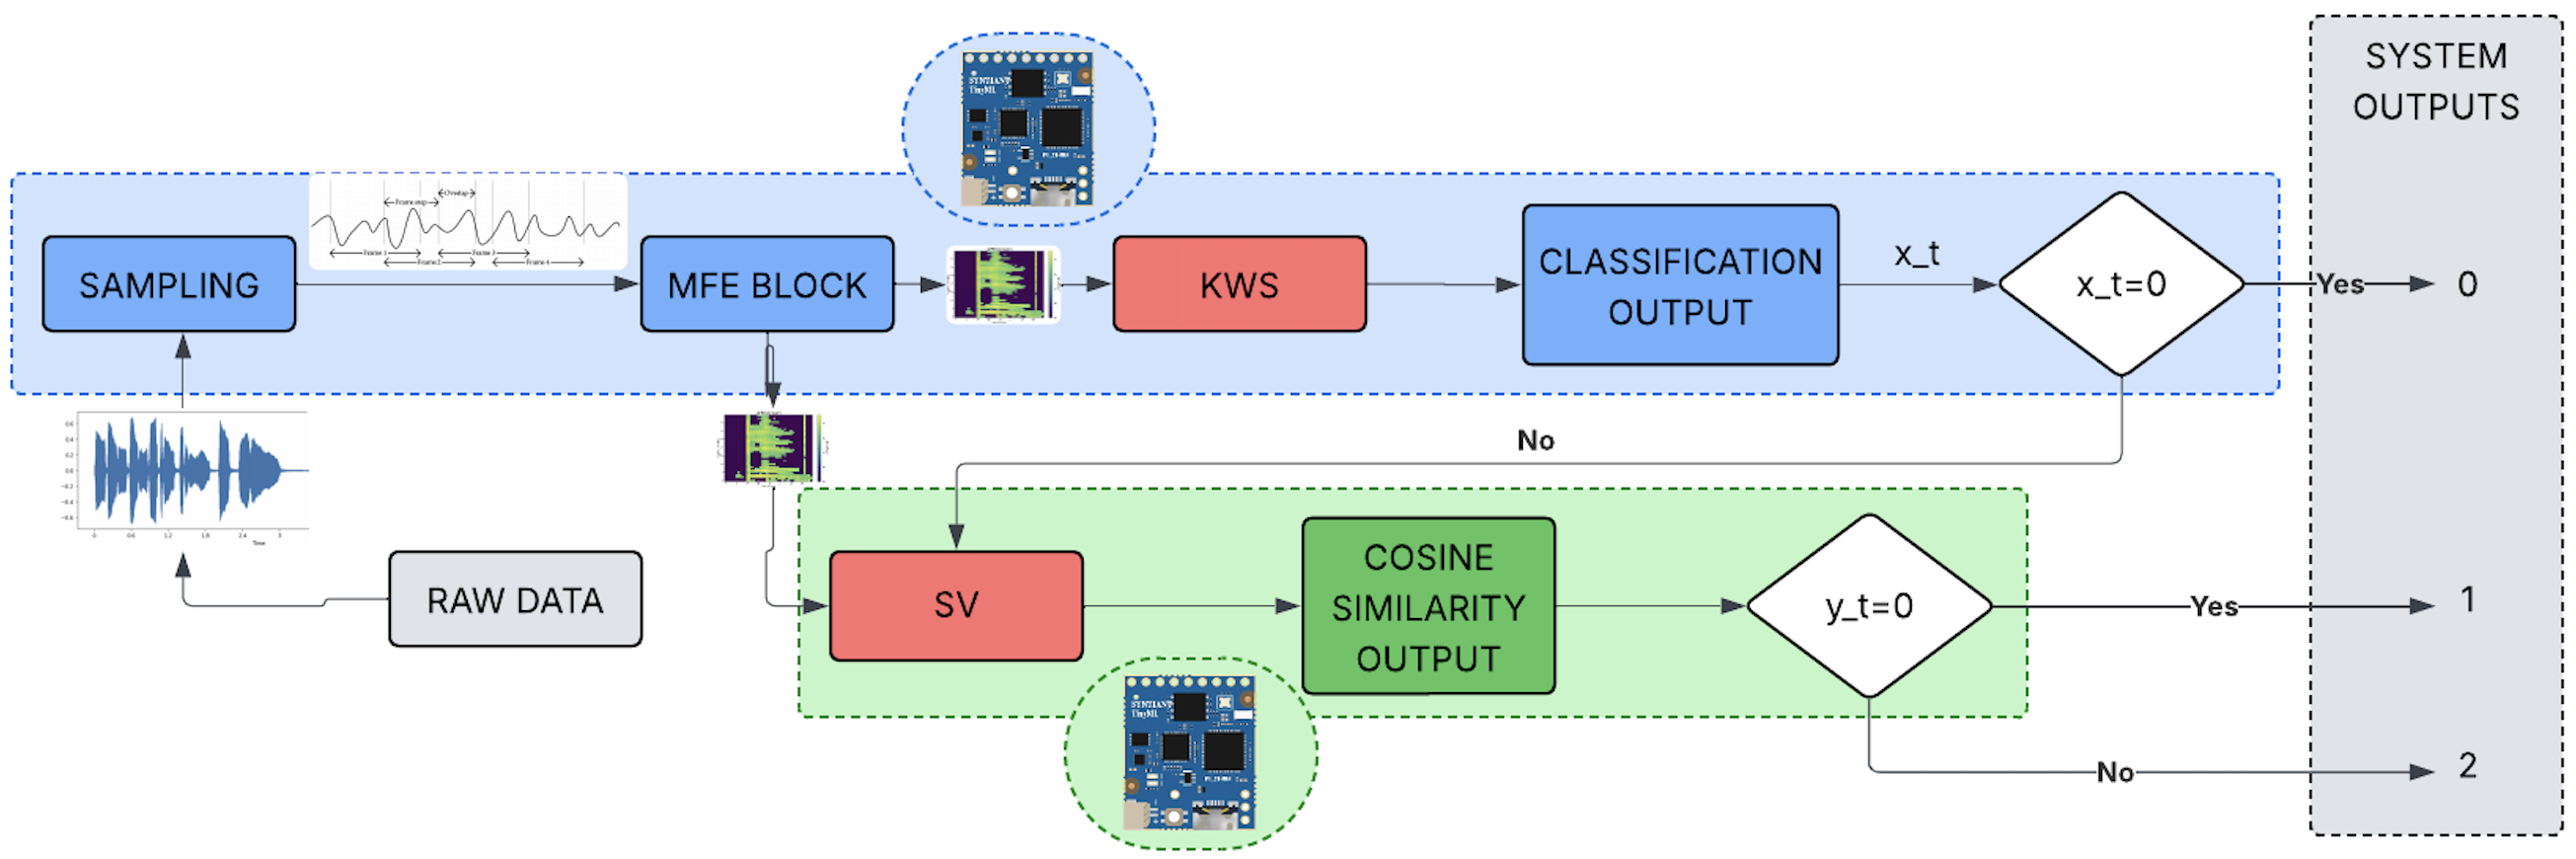
\includegraphics[width=1.0\textwidth]{images/4.01 Software Pipeline.png}
        \caption{Software Pipeline}
        \label{fig:software pipeline}
    \end{figure}
\end{center}
\section{Software Pipeline}
\label{sec:sw pipeline}
The system was developed in simulation and in validation using a simulation software approach, instead in inference only the code logic inside the single NDP101 was developed. In this section, we will talk about:\newline
• Signal Capture (Simulation)\newline
• MFE Block Generation and Processing (Simulation)\newline
• Model processing (Simulation)\newline
• Output Elaboration (Simulation+Inference)\newline
• Enrollment (Simulation+Inference)
\subsection{Signal Capture}
\label{subsec:signal}
The model requires real sampled raw data to work. If in Syntiant NDP101 there is a dual microphone integrated that computes the ADC conversion, three different modes were created on software to handle the code, according to the needs:\newline\newline
1. Live Sampling Mode (Mode 0) - The performing of live sampling from real input was performed to do fast debug, without the need to upload and create different files each time. The idea is to be a one-shot code, so when launched it activates the audio capture for one second and then uses that input audio as if it were the raw data inputted by the microphone. To do it, an external library called PortAudio\cite{portaudio}, which manages the input audio flow, starts it, stops it, and then calls a callback function to trigger the rest of the system.\newline
2. Files with .wav extension (Mode 1) - To perform validation, like a confusion matrix, multiple files should be parsed, which could not be done with live sampling. The idea was to create this mode that takes in input a .wav file that, with appropriate manipulation, would give the same output as PortAudio, but it can be reiterated. More precisely, using a bash file can be given in input a folder and the program will be called several times equal to the .wav files present in it. However, at the same time, it can be parsed as a single file. This is the primary technique used in the validation of graph performance model.\newline
3. Elaboration using data stored in a header (Mode 2) - The most primitive technique among the three proposed, but was useful in code creation and verification, and it consists of copying and pasting the digital values into a header file.\newline\newline
The properties of the audio computation were adapted from Syntiant, and for easiness sampled one second and then truncated the last 0.032 seconds, to have all samples long 0.968 seconds, which with a frequency of 16kHz, corresponds to 15488 digital elements.
\subsection{MFE Block Generation and Processing}
\label{subsec:mfe}
Previously, the theoretical and mathematical computation of the Syntiant block, which is similar to the MFE Block, was introduced with passages consisting of preemphasis, framing, mel-filterbanks, and noise floor. The code follows the mathematical logic, however, to support Fast Fourier Transformation, to be sure in using a functional and optimized code was used FFTW library, which has already implemented functions for Fast Fourier Transformation\cite{FFTW}. To verify the correct computation and application of the theoretical concepts, I relied on the Edge Impulse code\cite{edgeimpulse_processing_blocks}. This is a site on which deployment can be easily performed and provides a tool to convert input raw data to spectrogram features compatible with Syntiant NDP101. However, the Syntiant block code is not fully available and requires a trial-and-error implementation. To be sure that the code was corrected, a viewing validation was performed because Edge Impulse gives as output a visual spectrogram, so a Python code was implemented and called via a bash file after program computation that prints out the spectrogram features obtained, adjusting values until the two images matched or were very similar, as in \textbf{Figure \ref{fig:edgeimpulsespectrogram}} and \textbf{Figure \ref{fig:myspectrogram}}. The pseudocode for the logic is present in \textbf{Algorithm \ref{algorithm:spectrogram}}.
\begin{figure}[!h]
    \centering
    \begin{subfigure}[t]{0.4\textwidth}
        \centering
        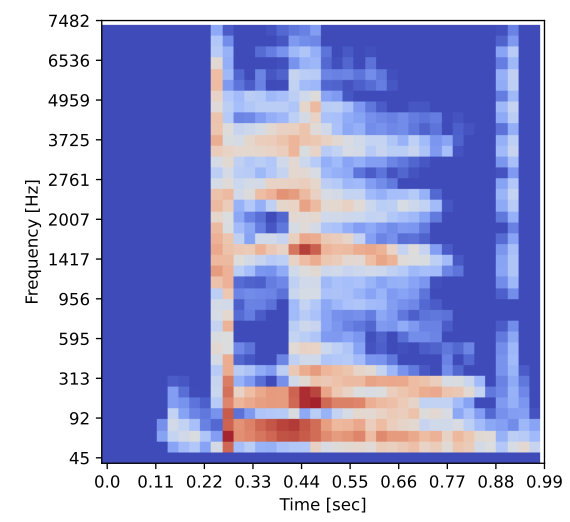
\includegraphics[width=\textwidth]{images/4.02 Spectrogram Edge Impulse.png}
        \caption{Edge Impulse Spectrogram}
        \label{fig:edgeimpulsespectrogram}
    \end{subfigure}
    \hfill
    \begin{subfigure}[t]{0.5\textwidth}
        \centering
        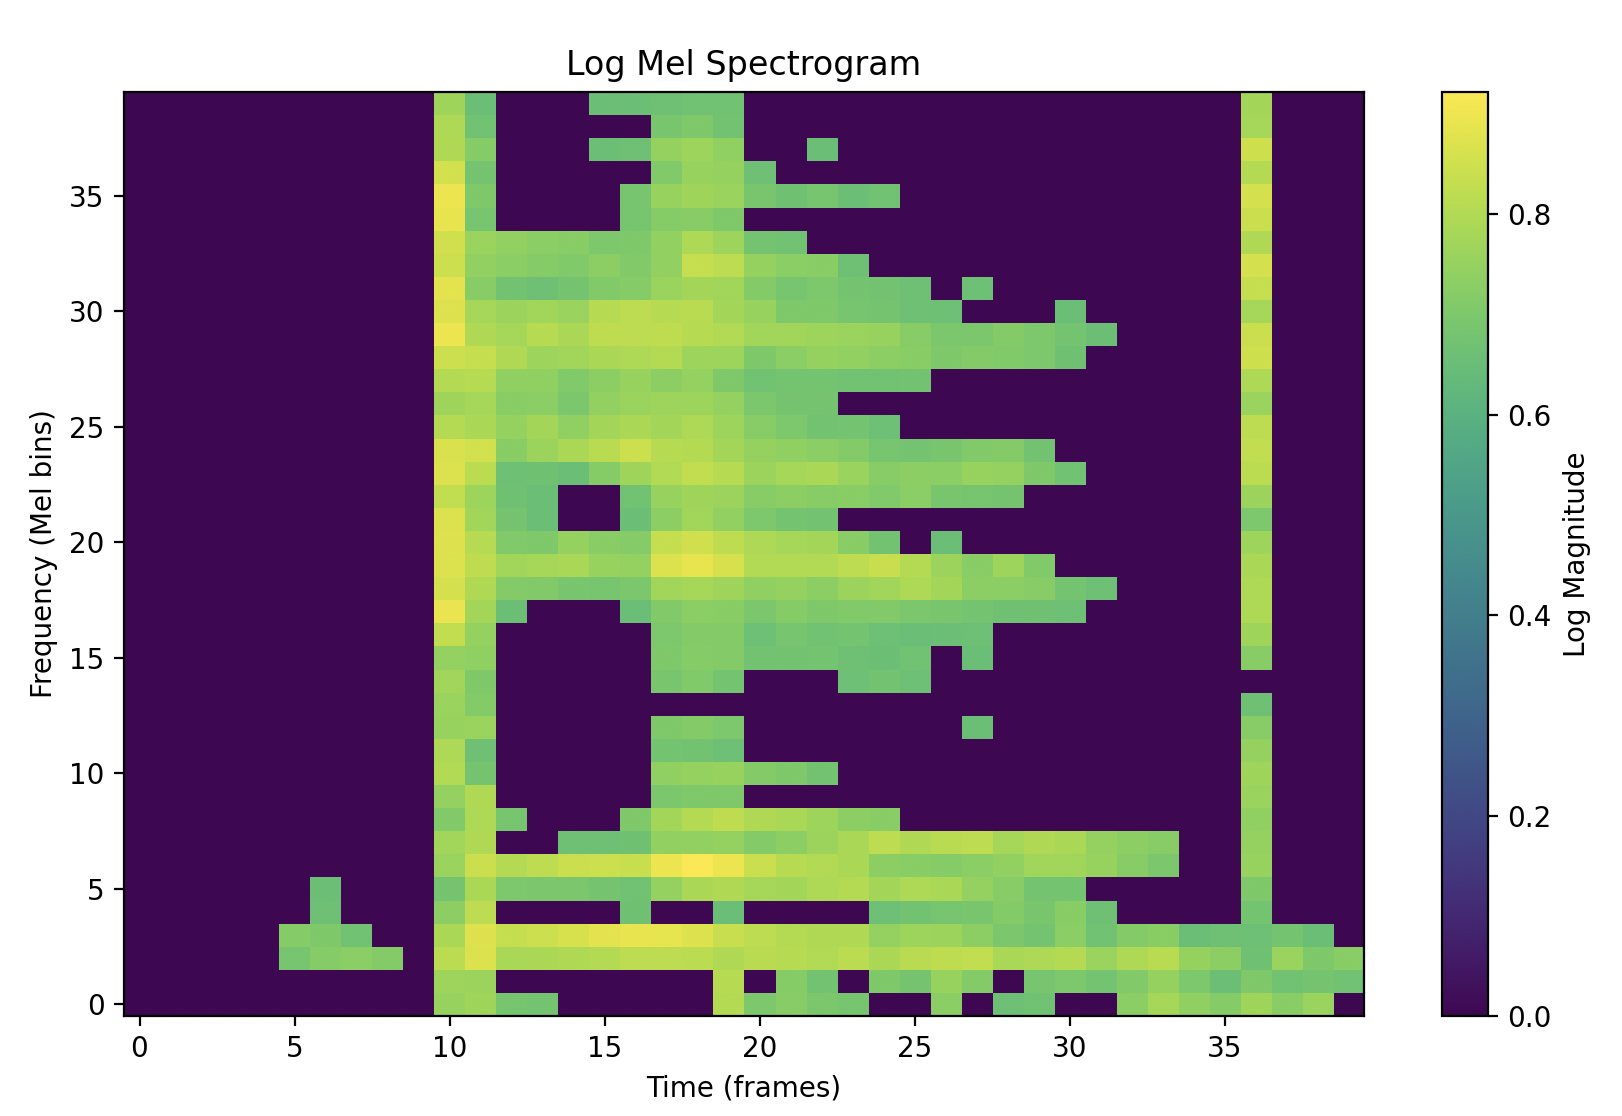
\includegraphics[width=\textwidth]{images/4.03 Spectrogram My Code.png}
        \caption{Custom Code Spectrogram}
        \label{fig:myspectrogram}
    \end{subfigure}
    \caption{Comparison of Spectrograms}
\end{figure}

\begin{algorithm}[H]
\caption{Spectrogram Computation Pipeline}
\label{algorithm:spectrogram}
\KwIn{Raw audio signal \texttt{audio[\,]} with \texttt{num\_samples} samples}
\KwOut{Log-Mel spectrogram \texttt{log\_mel\_spectrogram[\,]}}
\nl Normalize and apply pre-emphasis:\;
\Indp
    \For{$i \gets 0$ \KwTo $num\_samples - 1$}{
        $norm[i] \gets audio[i] / 32768.0$\;
    }
    $pre\_emphasis\_array[0] \gets norm[0]$\;
    \For{$i \gets 1$ \KwTo $num\_samples - 1$}{
        $pre\_emphasis\_array[i] \gets norm[i] - \texttt{COEFFICIENT} \times norm[i - 1]$\;
    }
\Indm
\nl Slice into overlapping frames and apply Hamming window:\;
\Indp
    \ForEach{frame $f$}{
        $fft\_in \gets$ frame of size \texttt{FRAME\_SIZE} from $pre\_emphasis\_array$\;
        \For{$i \gets 0$ \KwTo \texttt{FRAME\_SIZE} $- 1$}{
            $fft\_in[i] \gets fft\_in[i] \times (0.54 - 0.46 \times \cos(2\pi i / (FRAME\_SIZE - 1)))$\;
        }
\Indm
\nl Compute FFT and magnitude spectrum:\;
\Indp
        $fft\_out \gets \texttt{FFT}(fft\_in)$\;
        \For{$b \gets 0$ \KwTo \texttt{NUM\_BINS} $- 1$}{
            $spectrogram[f][b] \gets \sqrt{fft\_out[b].r^2 + fft\_out[b].i^2}$\;
        }
    }
\Indm
\nl Construct Mel filterbank:\;
\Indp
    Generate $FILTER\_NUMBER + 2$ evenly spaced Mel points between $MIN\_FREQ$ and $MAX\_FREQ$\;
    Convert Mel points to Hz and bin indices\;
    \ForEach{filter $j$}{
        Construct triangular filter between left, center, and right bins\;
        Assign weights to $mel\_filterbank[j][\,]$\;
    }
\Indm
\nl Apply Mel filters and compute log-Mel spectrogram:\;
\Indp
    \ForEach{frame $f$}{
        \ForEach{filter $j$}{
            $sum \gets \sum_k spectrogram[f][k] \times mel\_filterbank[j][k]$\;
            $log\_mel\_spectrogram[f][j] \gets 10 \times \log_{10}(sum + \varepsilon)$\;
        }
    }
\Indm
\nl Apply noise floor and quantization:\;
\Indp
    \ForEach{value in $log\_mel\_spectrogram$}{
        Normalize with respect to $NOISE\_FLOOR$\;
        Quantize to range $[0, 255]$, then normalize to $[0, 1]$\;
        Zero out values $< 0.65$\;
    }
\Indm
\KwRet{$log\_mel\_spectrogram$}
\end{algorithm}
\subsection{Models Processing}
The software pipeline first inferences the KWS model and, according to the result, if higher than 0, triggers the SV one. In simulation, they are handled with the components of the neural network explicitly shown. To weights and biases shall be declared to recall. At the same time, the input and output allocation of each layer should be allocated with respect to the functions that were created, the reasoning of the fully connected layer process, and the corresponding activation functions. The Syntiant model elaboration code for both the KWS and SV models follows the \textbf{Algorithm \ref{algorithm:neural network inference}}\footnotemark{}\footnotetext{Note that this is a general processing of a model because in the case shown KWS performs a softmax needed for classification, but it is not mandatory, for example SV performs only a ReLU. In the algorithm, the KWS is shown but has to be adapted to the needs of the user's model}, following the theoretical concepts.\newline
\begin{algorithm}[H]
\caption{Neural Network Inference Example}
\label{algorithm:neural network inference}
\KwIn{Input vector $x \in \mathbb{R}^{\texttt{INPUT\_SIZE}}$}
\KwOut{Predicted class index $y$}

\textbf{Initialize:} \\
\Indp
Create hidden layer buffers:
$fc_1 \in \mathbb{R}^{H_1}, \;
fc_2 \in \mathbb{R}^{H_2}, \;
fc_3 \in \mathbb{R}^{H_3}, \;
output \in \mathbb{R}^{C}$ \;
\Indm

\textbf{Feedforward pass:} \\
\Indp
$fc_1 \gets \texttt{ReLU}(W_1 x + b_1)$ \;
$fc_2 \gets \texttt{ReLU}(W_2 fc_1 + b_2)$ \;
$fc_3 \gets \texttt{ReLU}(W_3 fc_2 + b_3)$ \;
$output \gets \texttt{ReLU}(W_4 fc_3 + b_4)$ \;
\Indm

\textbf{Softmax normalization (if classification needs):} \\
\Indp
$\texttt{softmax}(output)$ \;
\Indm

\textbf{Sort and classify:} \\
\Indp
Sort $output$ in descending order, track original indices \;
Print top-$C$ class probabilities and names \;
\Indm

\Return{index of class with highest score}
\end{algorithm}

\subsection{Output Processing}
After the model elaborates its output the result should take several directions, for the KWS model classification method consists simply of using the output class to perform the desired action, like triggering the SV model, and can be simply done with an if-case in simulation and with SPI sending in inference, but different case is for SV model. To evaluate the result, a cosine similarity approach is used, consisting of comparing two different reference d-vectors to find a percentage of how much they are similar. Two different techniques of using reference features were explored in the previous chapter, but to compute the similarity to a mathematical formula consisting of the scalar product of the two vectors long N, divided by the product of their Euclidean norms:\newline
\begin{equation}
    cosine\_similarity(x,y)=\frac{x\cdot y}{|x|\cdot|y|}=\frac{\sum_{i=0}^{N}x_iy_i}{\sqrt{\sum_{i=0}^{N}x_i^2}\cdot\sqrt{\sum_{i=0}^{N}y_i^2}}
\end{equation}
This will be done among reference samples using the techniques of best-matching and mean-reference, previously introduced. So, after the comparison with the d-vector stored in the dataset according to the system threshold, the result will be binary: 0, if a d-vector similar to the one given in input in the dataset was not found, and 1 if yes.\newline
The structure of the dataset is first cataloged by words, then by user, and finally, per user's sample, if using the benchmatching technique. This system simplifies the overall computation, reducing the number of reference d-vectors to compare with the input one, simply giving the allocation in memory corresponding to the word selected and all the samples will be in a contiguous memory allocation to use spatial property, accessing only to the subsequent element, and uses information that it should receive anyway. Another consideration is that if a sample receives a similarity above the threshold, the system exists directly, and to output 0 it should parse all samples associated with the word given by KWS. The behavior is like the one in \textbf{Figure \ref{fig:dvector processing}}\newline
\begin{center}
    \centering
    \begin{figure}[!h]
        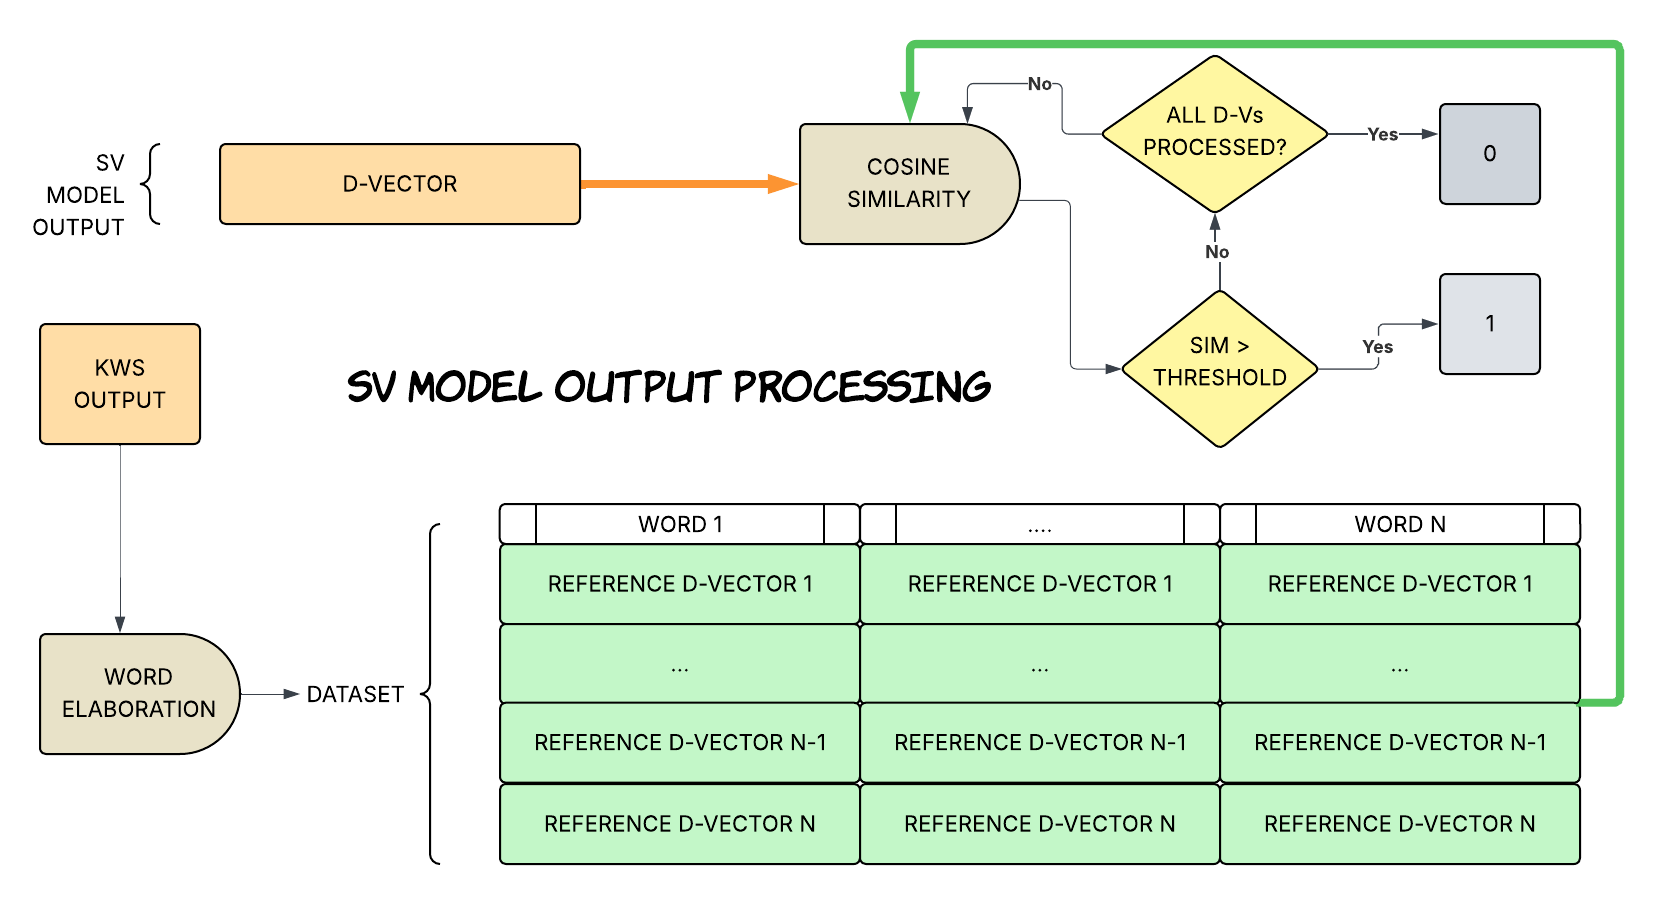
\includegraphics[width=1.0\textwidth]{images/4.04 D-Vector Processing.png}
        \caption{D-Vector Processing according to Database}
        \label{fig:dvector processing}
    \end{figure}
\end{center}
\subsection{Enrollment phase}
\label{subsec:enrollment} 
On inference, the complete application of this method is restricted due to the impossibility of quantizing the model to 4-bit precision and manipulating SPI interfaces. This limitation is primarily due to the nondisclosure agreement (NDA) surrounding the Syntiant NDP101, which prevents direct control over its internal functions. However, the Speaker Verification (SV) model was trained on a large and diverse dataset to generate a distinct d-vector representation for each user, enabling a one-time training process. In this scenario, the user needs to enroll by providing several voice samples. This number should be balanced: not too large to avoid excessive memory usage, but sufficient to maintain good recognition accuracy. The idea is to reuse the existing pipeline by replacing only the SV model inference stage. When enrolling, the user specifies the desired keyword, after which the system begins recording. However, it only saves samples that trigger the Keyword Spotting (KWS) model. Once the required number of valid samples is collected, the d-vectors are stored sequentially in memory by determining the current end of the dataset and appending the new d-vectors accordingly.
The memory structure for the dataset is designed such that each keyword is allocated a fixed portion of memory. In addition, a separate structure tracks the number of samples collected per keyword. Since each d-vector has a fixed length, it becomes straightforward to calculate the memory offset for appending new vectors. In the simulation, this dataset resides in a header file for simplicity, whereas in the actual inference phase, only the logic has been implemented and the full system integration has not been completed due to the limitations in connecting with the KWS system on hardware. Ideally, the dataset would be stored directly in internal SRAM, taking into account its typical 256-byte size constraint. However, some microcontrollers (MCUs) support external SD card storage, which could be used as an alternative. Using a memory mapping technique to manage allocation could be effective even with larger memory sizes and is unlikely to significantly impact energy consumption. Nevertheless, internal storage is generally preferable and should be tailored based on the remaining available memory after code and global variable allocations. A best-matching approach, where multiple samples per user are stored and compared, typically yields higher accuracy, but consumes more memory. Alternatively, averaging the d-vectors into a single representative vector per user results in lower precision but significantly reduces memory usage as it eliminates the need for storing multiple individual vectors.
\section{Hardware Pipeline}
\label{sec:hw pipeline}
Viewing the system from a hardware perspective, it will be made up of 2 Syntiant NDP101, one being the master device and the other the slave. The MCUs are both always on-devices, so they are continuously capturing audio, but the device that is handling KWS will always process all its software pipeline, instead SV one requires a trigger because of it being a slave. Going on or not should be setup with a SPI communication, which on Syntiant is provided by a internal SDK tool, allowing to setup 4 out of the 5 GPIO ports. The benefits of using an SPI communication stay in no interruptions, during the data transfer, so it would be a continuous stream, allowing the master device to perform synchronous and serial communication with the device. Another reason why this is preferable is the scalability, because knowing that Syntiant NDP101 could not hold much memory, to avoid more energy consumption with an external memory, other Syntiant NDP101 may be used for different words and create an hardware logic to redirect the sample to the correct microcontroller. The ports' settings to allow for this communication are:\newline
• MOSI (Master Output/Slave Input) - line that sends data/trigger to the slave\newline
• MISO (Master Input/Slave Output) - line that slave uses to send data to the master\newline
• SCLK (Clock) - line for the clock signal\newline 
• SS/CS (Slave Select) - line to select which slave to send data to, allowing for the scalability\newline
The setup in practice is like the one in \textbf{Figure \ref{fig:hardware setup}}:\newline
\begin{center}
    \centering
    \begin{figure}[!h]
        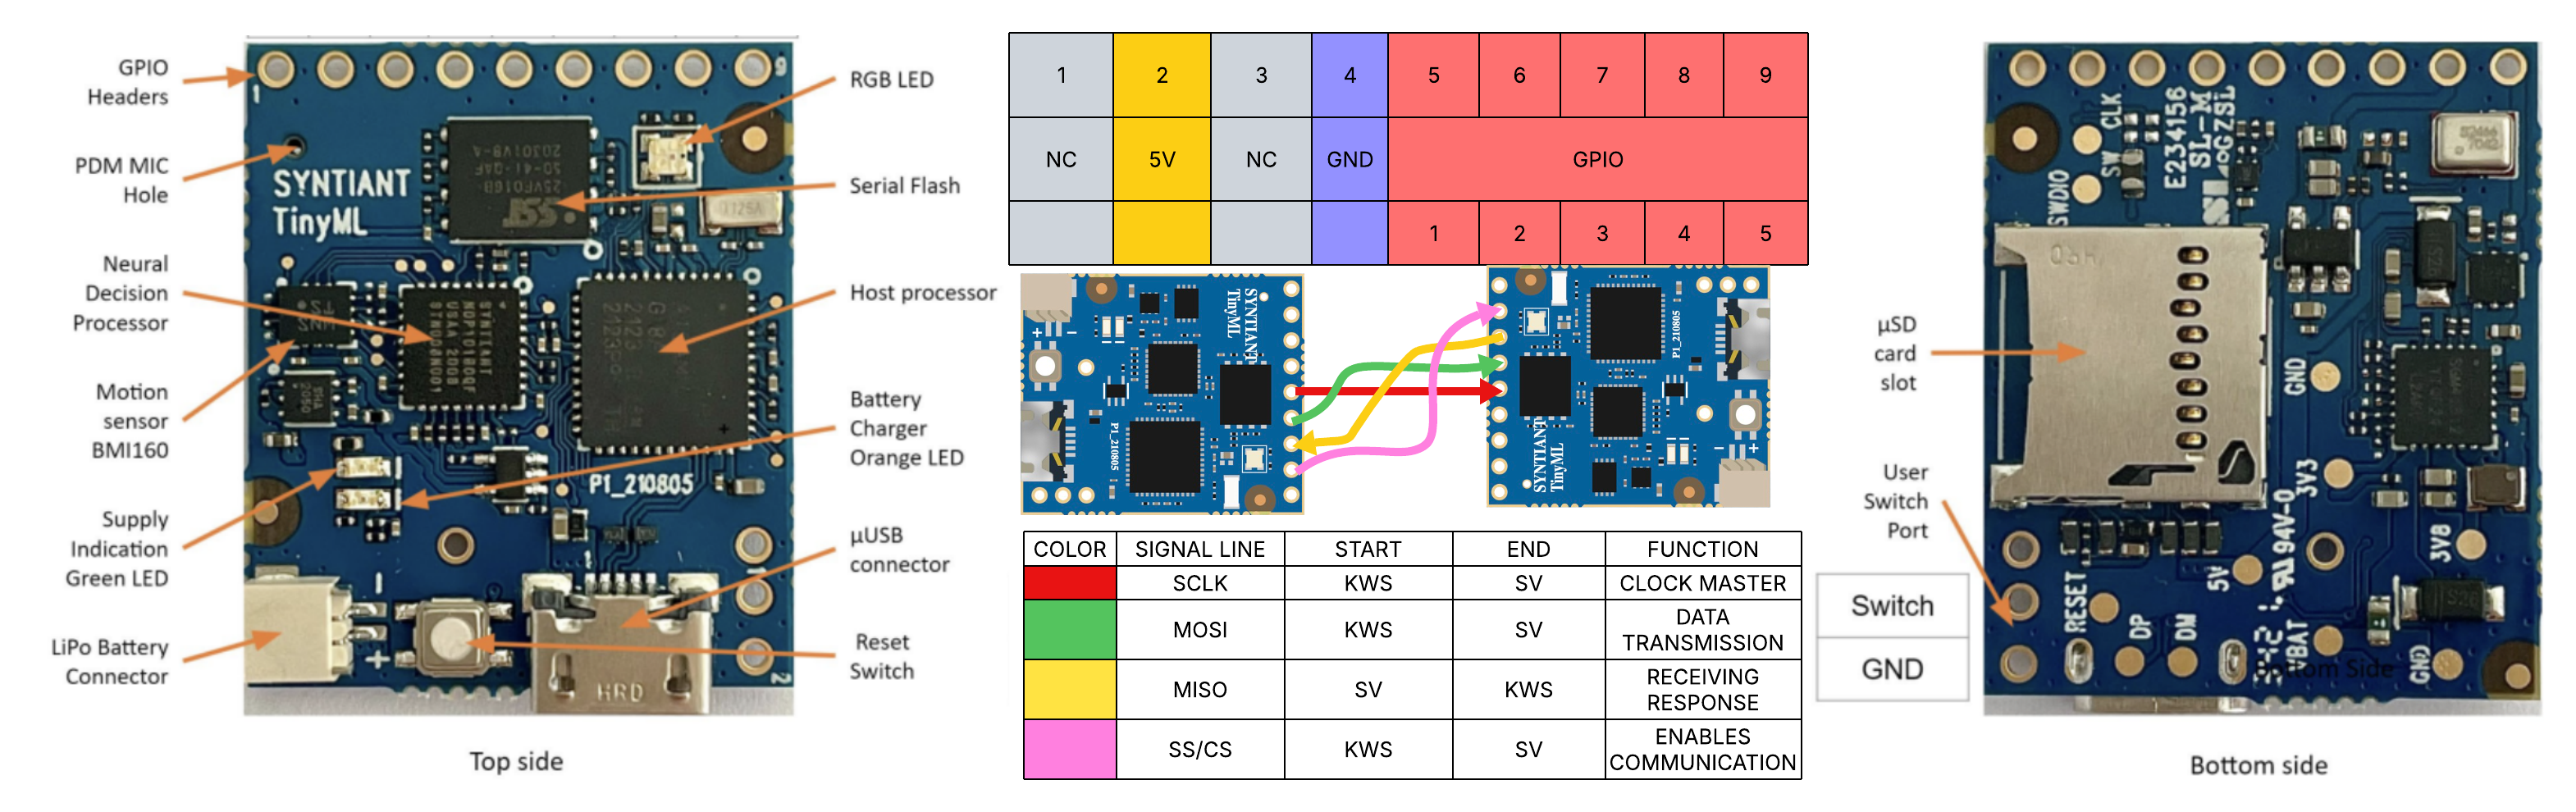
\includegraphics[width=1.0\textwidth]{images/4.05 Hardware Pipeline 2 NDP101.png}
        \caption{System Hardware Setup}
         \label{fig:hardware setup}
    \end{figure}
\end{center}
The pseudocode of each MCU consists in a setup function, called only once when the devices are turned on or after a reset and another that is continuously running and it is instead the core of the implementation.
The NDP101 is composed of sub-elements like the audio buffer that are not programmable, the only functions that can have some code uploaded can be the Flash Memory, to upload the trained AI model and the SRAM memory for the output management and other hardware component configuration.
The standard initialization of the microcontroller consists in loading the generated model, setting up the peripherals and the modalities, like low-power mode, to ensure the minimum energy consumption, so only when the microphone will recognize a distinguishable noise will it run the model. This is done via the WFI implementation (Wait For Interrupt), which handles in an efficient way the computation. When a relevant sound is detected, the peripherals are enabled again, and the interrupt NDP\_ISR is called. When the interrupt is triggered, the audio is automatically converted via the MFE block and gives the result as input to the model. If the model configuration and operations are directly in the binary file, the only thing that needs to be programmable is the output processing, distinguish the classification with a softmax activation function in KWS model case and a more composed logic with the dataset initialization, population, and comparison of d-vectors via cosine similarity introduced before. The code to perform both models on Syntiant has been written; however, was verified only for KWS, because of the inability of generating a model 4-int weight Syntiant compatible quantization for the SV model.
\newpage



